\chapter*{\textcolor{myred}{Epílogo}}

\textcolor{black}{\hrule}
\vspace{0.5cm}
{\huge{Conclusiones y Fronteras}}
\vspace{0.5cm}
\textcolor{black}{\hrule}

\newthought{Luego de haber realizado todo este recorrido por agujeros negros y espacio-tiempos curvados}, podemos afirmar que hemos aprendido mucho sobre Relatividad General. Ya sabemos interpretar muchas ecuaciones y métricas, e incluso hallar nuestras propias métricas para sistemas nuevos.

\vspace{0.5cm}

Uno de los resultados más interesantes a los que llegamos, que contradice bastante lo que estudiamos en Física III y Electromagnetismo I y II, es que aquí \textbf{los objetos con carga modifican las trayectorias de cualquier tipo de partícula}, independientemente de si esta última tiene carga o no. Esto es porque la fuente de la curvatura del espacio-tiempo es la \textbf{energía} (tensor de estrés-energía). Que un objeto sin carga pueda interactuar con un objeto con carga es un resultado análogo (e igual de sorprendente) a cuando un objeto sin masa -la \textbf{luz}- interactúa con un objeto con masa.

\vspace{0.5cm}

También fuimos capaces (no sin dificultad) de desarrollar un programa que realiza simulaciones de las trayectorias de partículas en un espacio-tiempo de Reisser-Nordström. Como esto es una generalización de espacio-tiempo de Schwarzschild, el programa también sirve para simular los problemas más conocidos de la Relatividad General: precesión del perihelio de Mercurio, deflección de la luz cerca de un objeto masivo. Incluso pudimos hacer una simulación del Sistema Solar.

\vspace{0.5cm}

Es posible expandir este trabajo realizando un estudio más minucioso del espacio-tiempo cerca del agujero negro de Reissner-Nordström, la presencia de carga eléctrica nos habilita a definir un nuevo radio, denominado \textbf{Radio de Cauchy}, que establece una región nueva entre dicho radio y el horizonte de eventos. Es posible analizar las diferencias entre cada una de las regiones del agujero negro. Este nuevo radio también nos permite postular la existencia de \textbf{singularidades desnudas}, que no tienen horizonte de eventos. Es decir, son agujeros 'negros' \textit{que dejan pasar la luz}.

\vspace{0.5cm}

Los agujeros negros con carga no existen en la realidad: para que los fenómenos aquí estudiados sean apreciables, necesitaríamos una carga del orden de los $10^{18}$ Coulomb. Sin embargo, el interés en este tipo de problemas no es puramente teórico: la métrica de Reissner-Nordström es el primer paso hacia la construcción de una métrica más general, que estudia los agujeros negros que rotan. Esta es la \textbf{métrica de Kerr}. Obviamente, una posible continuación del trabajo aquí realizado debería incorporar los agujeros negros de Kerr (y de Kerr-Newman, que rotan \textit{y} tienen carga eléctrica).

\vspace{0.5cm}

Por último, existe una rama de la Relatividad General llamada \textbf{gravitational lensing}, que estudia cómo la presencia de objetos masivos, al desviar la luz proveniente de estrellas lejanas, modifica las imágenes que pueden observarse desde la Tierra. Esto nos invita a utilizar técnicas computacionales de raytracing para simular cómo se vería un agujero negro.

\begin{figure}
    \centering
    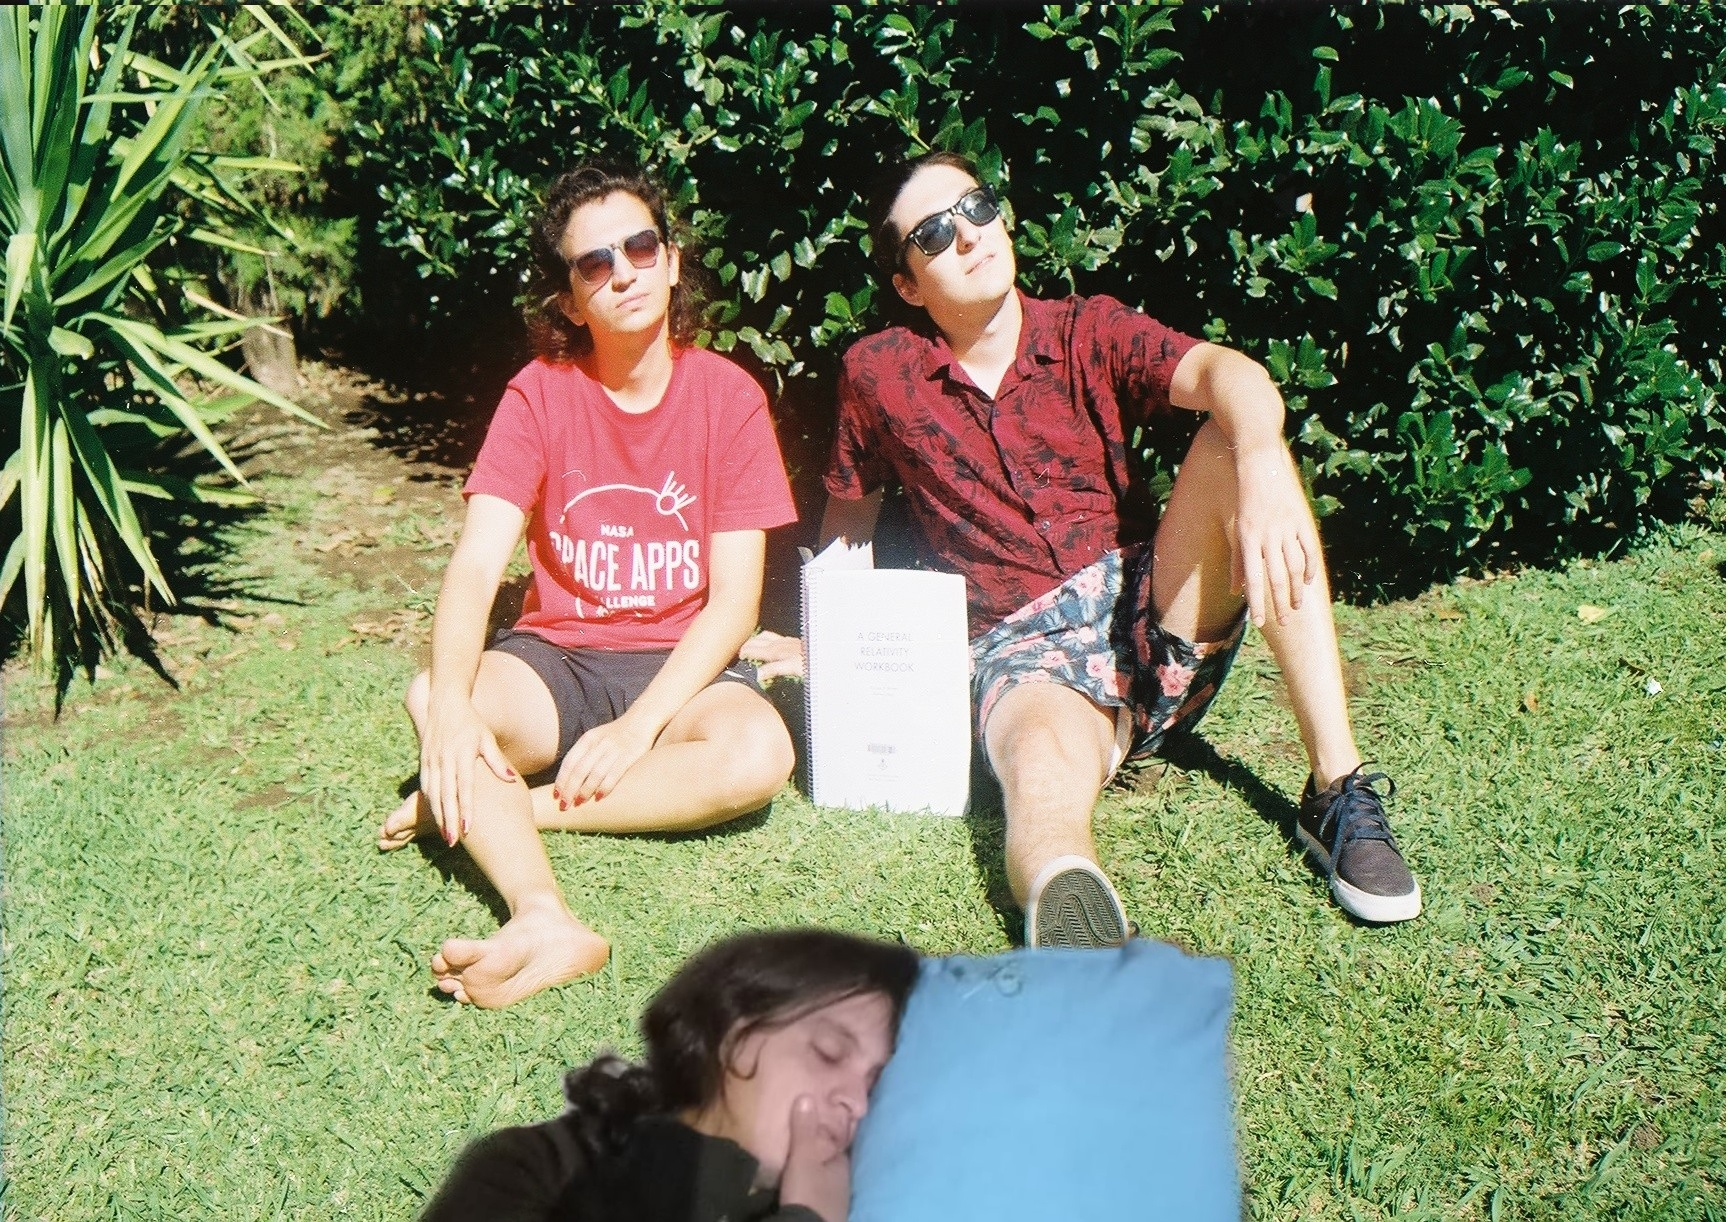
\includegraphics[width=\textwidth]{Im/F1000033-01.jpeg}
    \caption{Amigues relativistas.}
    \label{fig:my_label}
\end{figure}

\newpage
\textcolor{black}{\hrule}
\vspace{0.5cm}
{\huge{Material de Estudio}}
\vspace{0.5cm}
\textcolor{black}{\hrule}


\newthought{A continuación}, vamos a realizar un breve recorrido por los distintos recursos que utilizamos para estudiar estos temas.

\subsection*{\textbf{A General Relativity Workbook}, de Thomas A. Moore}
Este fue nuestro libro de cabecera, y tal como su nombre lo indica, es un libro diseñado para trabajar. Los capítulos tienen entre 5 y 10 páginas de extensión, y la mitad de los temas que desarrolla son propuestas para que resuelva lx estudiante. Abarca todos los temas relevantes para un primer curso de Relatividad General, y utiliza conceptos claros y sintéticos. 
\begin{marginfigure}
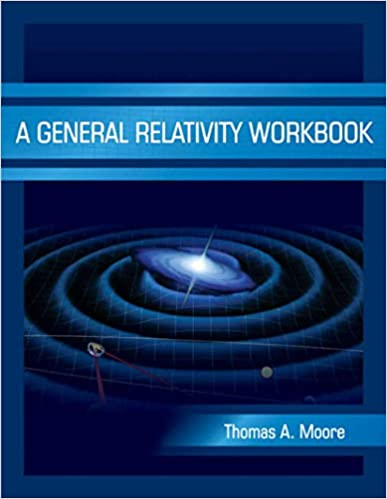
\includegraphics[width=0.8\textwidth]{Im/moore.jpg}
\end{marginfigure}

El libro no deja ningún término matemático sin definir, lo cual es ideal para quienes necesitan ver las cuentas para terminar de asimilar un tema (como nosotrxs). Es muy útil como guía conductora, aunque a veces no indaga tanto en lo conceptual para \textit{sacarle el jugo} a los temas.

\subsection*{\textbf{Exploring Black Holes: An Introdution to General Relativity}, de John A. Wheeler y Edwin F. Taylor}

Si en libro anterior tenía mucha matemática y poca interpretación, este libro es todo lo contrario. Sin mencionar tensores ni diferenciación covariante en ningún momento, los autores proponen trabajar con métricas 'dadas' y estudiar al máximo (\textit{explorar}) cómo es la geometría del espacio-tiempo. 
\begin{marginfigure}
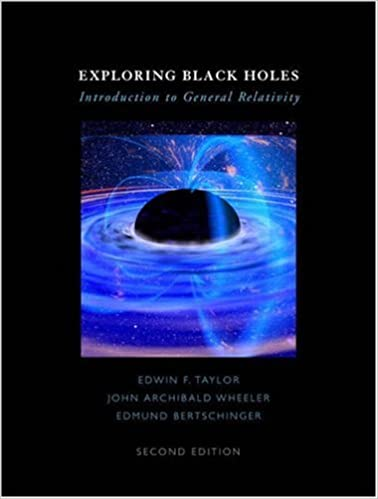
\includegraphics[width=0.8\textwidth]{Im/wheeler.jpg}
\end{marginfigure}
De a ratos puede parecer que todo está un poco \textit{en el aire}, en especial para quienes, al igual que nosotrxs, prefieren libros un poco más matemáticos. 

Algo muy interesante es la cantidad de proyectos que propone el libro. De hecho, la mitad del libro son instrucciones muy detalladas para resolver dichos proyectos. Fue el primer libro que encontramos sobre RG, porque justamente estábamos buscando proyectos guiados para resolver.

\subsection*{\textbf{The Classical Theory of Fields}, de Landau y Lifshitz}


Este libro no requiere demasiada introducción: para algunas personas es un \textit{ladrillo}, mientras que para otras es una \textit{caricia al alma}. 
\begin{marginfigure}
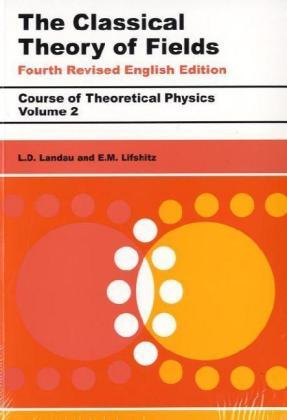
\includegraphics[width=0.8\textwidth]{Im/landau.jpg}
\end{marginfigure}
Lo cierto es que es un libro ideal para agarrar una vez que ya manejamos un poco los temas (lo mismo sucede con todos los libros de la serie de Landau), ya que no se priva de nada: tiene todo el formalismo matemático correspondiente a RG \textit{y} es conceptualmente profundo.
Sin dudas es un buen libro para consultar dudas, y en los primeros capítulos nos sirvió para tomar un hilo conductor.

\newpage

\subsection*{\textbf{Clases de Stanford} de Leonard Susskind}

Esta serie de 10 clases es ideal para ver los alcances que tiene la RG, explicados por una persona que lleva muchos años en el tema.
\begin{marginfigure}
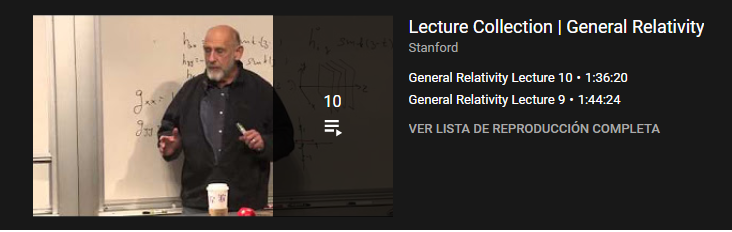
\includegraphics[width=1.3\textwidth]{Im/susskind.png}
\end{marginfigure}
Creo que se pueden apreciar mejor después de haber leído los capítulos 3 a 6 y 17 a 19 del Moore, ya que Susskind casi no escribe en el pizarrón y a veces es difícil seguir los conceptos matemáticos más abstractos sin una buena representación visual. Es ideal para estudiar qué sucede en un agujero negro de Schwarzschild y para introducirse en los Diagramas de Penrose.

\subsection*{\textbf{Einstein Field Equations For Beginners!} de DrPhysicsA}

Este video es la manera perfecta de spoilearse RG desmenuzando las Ecuaciones de Einstein. Todo el video está hecho en una hoja de papel y narrado por una voz con un acento muy inglés. 
\begin{marginfigure}
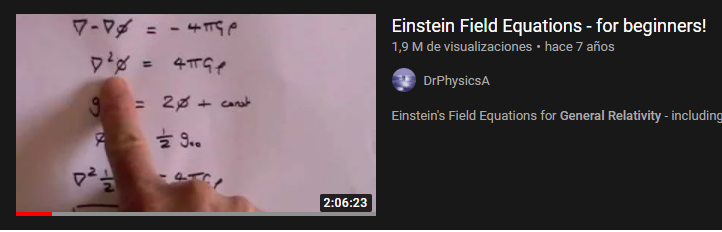
\includegraphics[width=1.3\textwidth]{Im/bumpyy.png}
\end{marginfigure}
Creo que es una buena manera de hacer un pantallazo general de los temas, ya que es muy fácil de entender y nos presenta todos los elementos que vamos a tener que utilizar más adelante.

\subsection*{\textbf{Your Daily Equation} de Brian Greene}

A partir del episodio 26, el autor de \textbf{The Elegant Universe} comienza a explicarnos las Ecuaciones de Campo de Einstein y todos los elementos que la constituyen.
\begin{marginfigure}
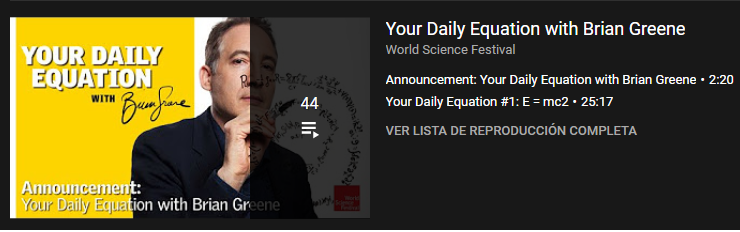
\includegraphics[width=1.3\textwidth]{Im/bumpy.png}
\end{marginfigure}
Da muchos ejemplos para hacer entender los conceptos, y de ahí sacamos gran parte de la sección \textit{GR In a Nutshell} de este apunte.

\subsection*{\textbf{The Maths of General Relativity} de Science Clic}

Esta es una serie de 8 videos que empezó a subirse a finales de 2020 y fue terminada en enero de 2021. Las animaciones están muy bien hechas y permiten entender varios conceptos de manera rápida y clara. 

Se complementa muy bien con libros como el Moore o el Landau, ya que en una animación de 15 segundos sintetiza lo que Landau puede estar dos páginas enteras explicando sin usar una sola imagen.
\begin{marginfigure}
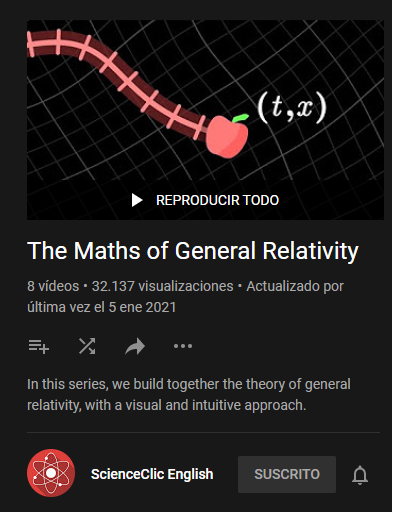
\includegraphics[width=1.3\textwidth]{Im/scienceclic.png}
\end{marginfigure}

\begin{marginfigure}

\includegraphics[width=0.8\textwidth]{Im/qr_img.png}
\end{marginfigure}
\vspace{4cm}
\newthought{En el siguiente link}, encontrarán toda información relacionada con este trabajo, así como también los códigos que hicimos para realizar las simulaciones y varios videos de dichas simulaciones.

\textcolor{myred}{\underline{\url{https://drive.google.com/drive/folders/1AZ_T-1sP442UiVBRkR45JsUwid0Mn6Qu?usp=sharing}}}

